\begin{figure}
    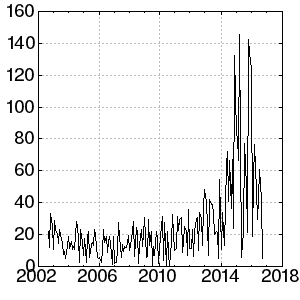
\includegraphics[scale=0.65]{../scripts/refugees_war_rand/refugees_rand.png}
    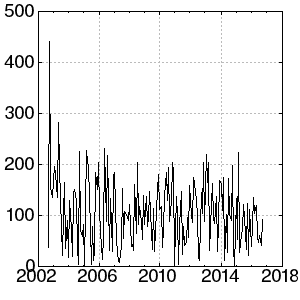
\includegraphics[scale=0.65]{../scripts/refugees_war_rand/war_rand.png}
    \caption{Grafikas kairėje: užtriukšmintas vidutinis mėnesinis karo pabėgėlių skaičius pasaulyje (tūkstančiais). Grafikas dešinėje: užtriukšmintas mėnesinis „war“ skaičius ABC naujienų antraštėse.}
    \label{fig:noisy}
\end{figure}

\begin{figure}
    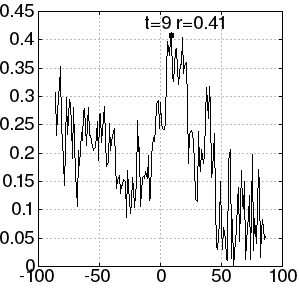
\includegraphics[scale=0.65]{../scripts/refugees_war_rand/result_ref_rand.png}
    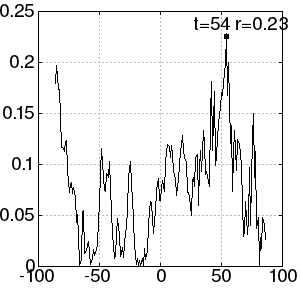
\includegraphics[scale=0.65]{../scripts/refugees_war_rand/result_war_rand.png}
    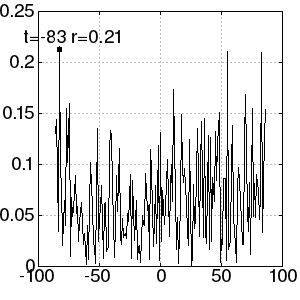
\includegraphics[scale=0.65]{../scripts/refugees_war_rand/result_both_rand.png}
    \caption{Grafikas kairėje: užtriukšminto pabėgėlių ir švaraus „war“ dažnumo koreliacija. Grafikas centre: švaraus pabėgėlių ir užtriukšminto „war“ dažnumo koreliacija. Grafikas dešinėje: signalų tarpusavio koreliacija kai abu signalai užtiukšminti}
    \label{fig:noisy_cross}
\end{figure}

Užtriukšminti karo pabėgėlių ir žodžio „war“ skaičius per mėnesį signalai (~\ref{fig:noisy} pav. ) gauti panaudojus paprastą 'random' generatorių \(y = x * rand(0, 1)\).

Iš koreliacijos grafikų (~\ref{fig:noisy_cross} pav. ) matosi, kad užtriukšmintas pabėgelių skaičius nestipriai pakeitė algoritmo rezultatus.
Bet užtriukšmintas „war“ dažnumas daug stipririau iškreipė koreliacijos grafiką.
Galiausiai, kai abu signalai užtriukšmniti, algoritmas neberanda koreliacijos tarp jų.
